\documentclass{standalone}
\usepackage{tikz}
\usetikzlibrary{patterns, positioning}
\usepackage[sfdefault]{ClearSans} %% option 'sfdefault' activates Clear Sans as the default text font
\usepackage[T1]{fontenc}

\begin{document}
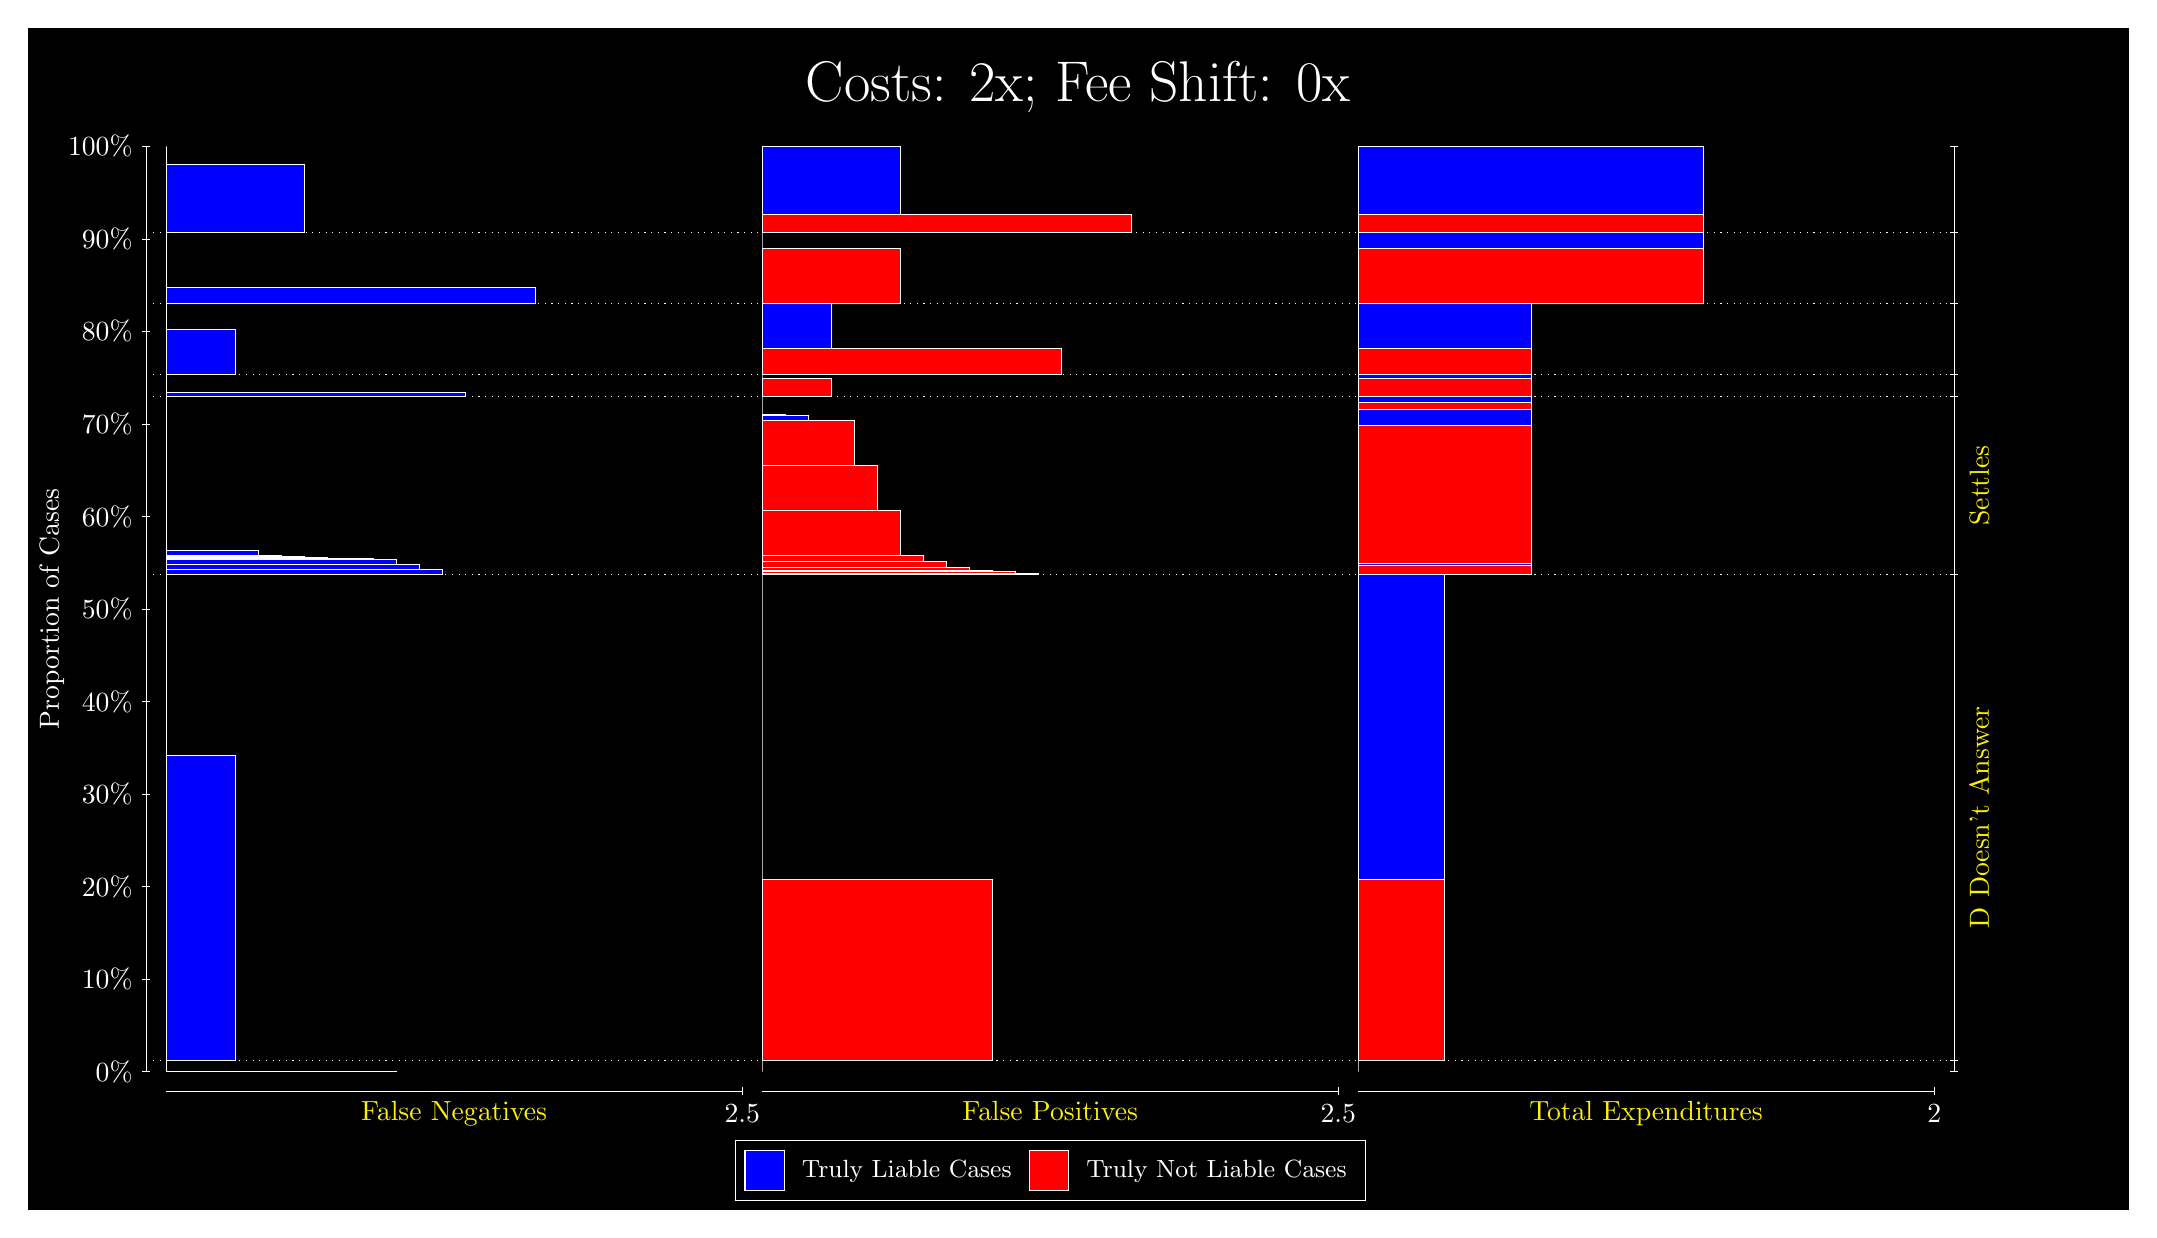
\begin{tikzpicture}
\draw[fill=black] (0,0) rectangle (26.667,15);
\draw[text=white] (0,13.5) rectangle (26.667,15) node[midway] {\huge Costs: 2x; Fee Shift: 0x};
\draw[white, very thin] (1.5,1.75) -- (1.5,13.5);
\node[rotate=90, text=white, anchor=center] at (0.3, 7.625) {Proportion of Cases};
\draw[white, very thin] (1.45,1.75) -- (1.55,1.75);
\node[text=white, anchor=east] at (1.45, 1.75) {0\%};
\draw[white, very thin] (1.45,2.925) -- (1.55,2.925);
\node[text=white, anchor=east] at (1.45, 2.925) {10\%};
\draw[white, very thin] (1.45,4.1) -- (1.55,4.1);
\node[text=white, anchor=east] at (1.45, 4.1) {20\%};
\draw[white, very thin] (1.45,5.275) -- (1.55,5.275);
\node[text=white, anchor=east] at (1.45, 5.275) {30\%};
\draw[white, very thin] (1.45,6.45) -- (1.55,6.45);
\node[text=white, anchor=east] at (1.45, 6.45) {40\%};
\draw[white, very thin] (1.45,7.625) -- (1.55,7.625);
\node[text=white, anchor=east] at (1.45, 7.625) {50\%};
\draw[white, very thin] (1.45,8.8) -- (1.55,8.8);
\node[text=white, anchor=east] at (1.45, 8.8) {60\%};
\draw[white, very thin] (1.45,9.975) -- (1.55,9.975);
\node[text=white, anchor=east] at (1.45, 9.975) {70\%};
\draw[white, very thin] (1.45,11.15) -- (1.55,11.15);
\node[text=white, anchor=east] at (1.45, 11.15) {80\%};
\draw[white, very thin] (1.45,12.325) -- (1.55,12.325);
\node[text=white, anchor=east] at (1.45, 12.325) {90\%};
\draw[white, very thin] (1.45,13.5) -- (1.55,13.5);
\node[text=white, anchor=east] at (1.45, 13.5) {100\%};

\draw[white, very thin] (24.457,1.75) -- (24.457,13.5);
\draw[white, very thin] (24.407,1.75) -- (24.507,1.75);
\node[anchor=west] at (24.407, 1.75) {};
\draw[white, very thin] (24.407,1.8911) -- (24.507,1.8911);
\node[anchor=west] at (24.407, 1.8911) {};
\draw[white, very thin] (24.407,8.0626) -- (24.507,8.0626);
\node[anchor=west] at (24.407, 8.0626) {};
\draw[white, very thin] (24.407,10.324) -- (24.507,10.324);
\node[anchor=west] at (24.407, 10.324) {};
\draw[white, very thin] (24.407,10.606) -- (24.507,10.606);
\node[anchor=west] at (24.407, 10.606) {};
\draw[white, very thin] (24.407,11.505) -- (24.507,11.505);
\node[anchor=west] at (24.407, 11.505) {};
\draw[white, very thin] (24.407,12.408) -- (24.507,12.408);
\node[anchor=west] at (24.407, 12.408) {};
\draw[white, very thin] (24.407,13.5) -- (24.507,13.5);
\node[anchor=west] at (24.407, 13.5) {};

\draw[white, very thin, fill=blue] (1.75,1.75) rectangle (4.6775,1.7583);
\draw[white, very thin, fill=red] (1.75,1.7583) rectangle (1.75,1.8911);
\draw[white, very thin, fill=blue] (1.75,1.8911) rectangle (2.6283,5.7632);
\draw[white, very thin, fill=red] (1.75,5.7632) rectangle (1.75,8.0626);
\draw[white, very thin, fill=blue] (1.75,8.0626) rectangle (5.2631,8.1266);
\draw[white, very thin, fill=blue] (1.75,8.1266) rectangle (4.9703,8.1901);
\draw[white, very thin, fill=blue] (1.75,8.1901) rectangle (4.6775,8.2535);
\draw[white, very thin, fill=blue] (1.75,8.2535) rectangle (4.3848,8.2581);
\draw[white, very thin, fill=blue] (1.75,8.2581) rectangle (4.3848,8.2622);
\draw[white, very thin, fill=blue] (1.75,8.2622) rectangle (4.092,8.272);
\draw[white, very thin, fill=blue] (1.75,8.272) rectangle (3.7993,8.2773);
\draw[white, very thin, fill=blue] (1.75,8.2773) rectangle (3.5065,8.2899);
\draw[white, very thin, fill=blue] (1.75,8.2899) rectangle (3.2138,8.3022);
\draw[white, very thin, fill=blue] (1.75,8.3022) rectangle (2.921,8.3675);
\draw[white, very thin, fill=red] (1.75,8.3675) rectangle (1.75,10.324);
\draw[white, very thin, fill=blue] (1.75,10.324) rectangle (5.5558,10.372);
\draw[white, very thin, fill=red] (1.75,10.372) rectangle (1.75,10.606);
\draw[white, very thin, fill=blue] (1.75,10.606) rectangle (2.6283,11.181);
\draw[white, very thin, fill=red] (1.75,11.181) rectangle (1.75,11.505);
\draw[white, very thin, fill=blue] (1.75,11.505) rectangle (6.4341,11.71);
\draw[white, very thin, fill=red] (1.75,11.71) rectangle (1.75,12.408);
\draw[white, very thin, fill=blue] (1.75,12.408) rectangle (3.5065,13.27);
\draw[white, very thin, fill=red] (1.75,13.27) rectangle (1.75,13.5);
\draw[white, very thin, fill=red] (9.3189,1.75) rectangle (9.3189,1.8828);
\draw[white, very thin, fill=blue] (9.3189,1.8828) rectangle (9.3189,1.8911);
\draw[white, very thin, fill=red] (9.3189,1.8911) rectangle (12.246,4.1905);
\draw[white, very thin, fill=blue] (9.3189,4.1905) rectangle (9.3189,8.0626);
\draw[white, very thin, fill=red] (9.3189,8.0626) rectangle (12.832,8.0808);
\draw[white, very thin, fill=red] (9.3189,8.0808) rectangle (12.539,8.0973);
\draw[white, very thin, fill=red] (9.3189,8.0973) rectangle (12.246,8.1169);
\draw[white, very thin, fill=red] (9.3189,8.1169) rectangle (11.954,8.1567);
\draw[white, very thin, fill=red] (9.3189,8.1567) rectangle (11.661,8.2333);
\draw[white, very thin, fill=red] (9.3189,8.2333) rectangle (11.368,8.3027);
\draw[white, very thin, fill=red] (9.3189,8.3027) rectangle (11.075,8.8765);
\draw[white, very thin, fill=red] (9.3189,8.8765) rectangle (10.783,9.4517);
\draw[white, very thin, fill=red] (9.3189,9.4517) rectangle (10.49,10.019);
\draw[white, very thin, fill=blue] (9.3189,10.019) rectangle (9.9044,10.084);
\draw[white, very thin, fill=blue] (9.3189,10.084) rectangle (9.6116,10.097);
\draw[white, very thin, fill=blue] (9.3189,10.097) rectangle (9.3189,10.324);
\draw[white, very thin, fill=red] (9.3189,10.324) rectangle (10.197,10.558);
\draw[white, very thin, fill=blue] (9.3189,10.558) rectangle (9.3189,10.606);
\draw[white, very thin, fill=red] (9.3189,10.606) rectangle (13.125,10.93);
\draw[white, very thin, fill=blue] (9.3189,10.93) rectangle (10.197,11.505);
\draw[white, very thin, fill=red] (9.3189,11.505) rectangle (11.075,12.203);
\draw[white, very thin, fill=blue] (9.3189,12.203) rectangle (9.3189,12.408);
\draw[white, very thin, fill=red] (9.3189,12.408) rectangle (14.003,12.638);
\draw[white, very thin, fill=blue] (9.3189,12.638) rectangle (11.075,13.5);
\draw[white, very thin, fill=red] (16.888,1.75) rectangle (16.888,1.8828);
\draw[white, very thin, fill=blue] (16.888,1.8828) rectangle (16.888,1.8911);
\draw[white, very thin, fill=red] (16.888,1.8911) rectangle (17.986,4.1905);
\draw[white, very thin, fill=blue] (16.888,4.1905) rectangle (17.986,8.0626);
\draw[white, very thin, fill=red] (16.888,8.0626) rectangle (19.083,8.1752);
\draw[white, very thin, fill=blue] (16.888,8.1752) rectangle (19.083,8.21);
\draw[white, very thin, fill=red] (16.888,8.21) rectangle (19.083,9.9631);
\draw[white, very thin, fill=blue] (16.888,9.9631) rectangle (19.083,10.159);
\draw[white, very thin, fill=red] (16.888,10.159) rectangle (19.083,10.249);
\draw[white, very thin, fill=blue] (16.888,10.249) rectangle (19.083,10.324);
\draw[white, very thin, fill=red] (16.888,10.324) rectangle (19.083,10.558);
\draw[white, very thin, fill=blue] (16.888,10.558) rectangle (19.083,10.606);
\draw[white, very thin, fill=red] (16.888,10.606) rectangle (19.083,10.93);
\draw[white, very thin, fill=blue] (16.888,10.93) rectangle (19.083,11.505);
\draw[white, very thin, fill=red] (16.888,11.505) rectangle (21.279,12.203);
\draw[white, very thin, fill=blue] (16.888,12.203) rectangle (21.279,12.408);
\draw[white, very thin, fill=red] (16.888,12.408) rectangle (21.279,12.638);
\draw[white, very thin, fill=blue] (16.888,12.638) rectangle (21.279,13.5);
\draw[white, dotted] (1.5,1.8911) -- (24.457,1.8911);
\draw[white, dotted] (1.5,8.0626) -- (24.457,8.0626);
\draw[white, dotted] (1.5,10.324) -- (24.457,10.324);
\draw[white, dotted] (1.5,10.606) -- (24.457,10.606);
\draw[white, dotted] (1.5,11.505) -- (24.457,11.505);
\draw[white, dotted] (1.5,12.408) -- (24.457,12.408);
\draw[white, very thin] (1.75,1.5) -- (9.0689,1.5);
\node[text=yellow, anchor=north] at (5.4094, 1.5) {False Negatives};
\draw[white, very thin] (9.0689,1.45) -- (9.0689,1.55);
\node[text=white, anchor=north] at (9.0689, 1.45) {2.5};

\draw[white, very thin] (9.3189,1.5) -- (16.638,1.5);
\node[text=yellow, anchor=north] at (12.978, 1.5) {False Positives};
\draw[white, very thin] (16.638,1.45) -- (16.638,1.55);
\node[text=white, anchor=north] at (16.638, 1.45) {2.5};

\draw[white, very thin] (16.888,1.5) -- (24.207,1.5);
\node[text=yellow, anchor=north] at (20.547, 1.5) {Total Expenditures};
\draw[white, very thin] (24.207,1.45) -- (24.207,1.55);
\node[text=white, anchor=north] at (24.207, 1.45) {2};


\node[text=yellow, centered, rotate=90] at (24.777, 4.9768) {D Doesn't Answer};
\node[text=yellow, centered, rotate=90] at (24.777, 9.1933) {Settles};





\draw (12.978300999999998,1.5) node[draw=none] (baseCoordinate) {};
\begin{scope}[align=center]
        \matrix[scale=0.5, draw=white, below=0.5cm of baseCoordinate, nodes={draw}, column sep=0.1cm]{
            \node[rectangle, draw, minimum width=0.5cm, minimum height=0.5cm, fill=blue] {}; &
            \node[draw=none, font=\small, text=white] (B) {Truly Liable Cases}; &
            \node[rectangle, draw, minimum width=0.5cm, minimum height=0.5cm, fill=red] {}; &
            \node[draw=none, font=\small, text=white] (B) {Truly Not Liable Cases}; \\
            };
\end{scope}

\end{tikzpicture}
\end{document}